%%%%%%%%%%%%%%%%%%%%%%%%%%%%%%%%%%%%%%%%%%%%%%%%%%%%%%%%%%%%%%%%%%%%%%
%%                     necessary stimulation
%%%%%%%%%%%%%%%%%%%%%%%%%%%%%%%%%%%%%%%%%%%%%%%%%%%%%%%%%%%%%%%%%%%%%%
\color{ForestGreen}

\subsubsection{Glyph: \glyph{Necessary stimulation}}\label{sec:necessaryStimulation}

A necessary stimulation is an influence that has to be present for a relationship to take place (to become true). A relationship modulated by a necessary stimulation can only exist when this stimulation is true, whatever are the other influences this relationship is subjected to.

\begin{glyphDescription}
 \glyphSboTerm SBO:0000171 ! necessary stimulation.
 \glyphOrigin Any \glyph{interactor} (\sect{interactors}) or any \glyph{logical operator} (\sect{logic}).
 \glyphTarget Any \glyph{statement} (\sect{statements}) or \glyph{influence} (\sect{influences}).
 \glyphEndPoint The target extremity of a \glyph{necessary stimulation} carries an open arrow (to remind that it is a \glyph{stimulation}) coming after a larger vertical bar.
 \end{glyphDescription}

\begin{figure}[H]
  \centering
  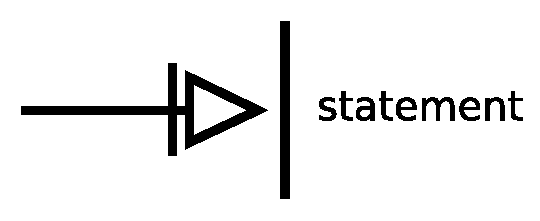
\includegraphics[scale = 0.5]{images/necessaryStimulation}
  \caption{The \PD glyph for \glyph{necessaryStimulation}.}
  \label{fig:necessaryStimulation}
\end{figure}

\begin{figure}[H]
  \centering
  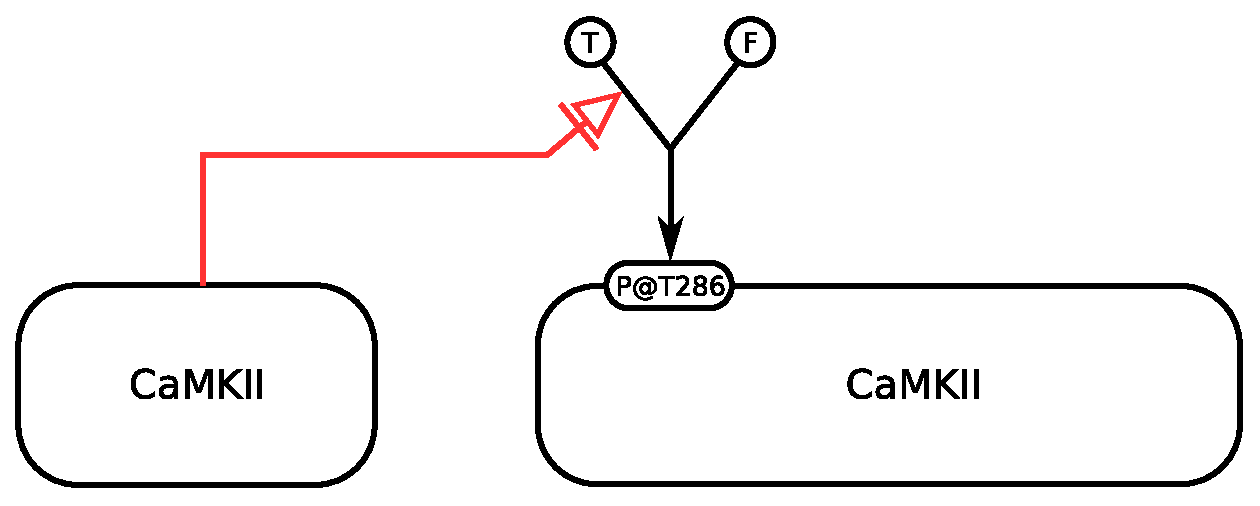
\includegraphics[scale = 0.5]{examples/ex-necessaryStimulation}
  \caption{This example shows how threonine 286 of CaMKII is only phosphorylated by the kinase itself, but in a trans-fashion, meaning a molecule of CaMKII does not phosphorylate itself, but another molecule of CaMKII.}
  \label{fig:ex-necessaryStimulation}
\end{figure}

\normalcolor